\documentclass{standalone}
\usepackage{tikz}


\begin{document}

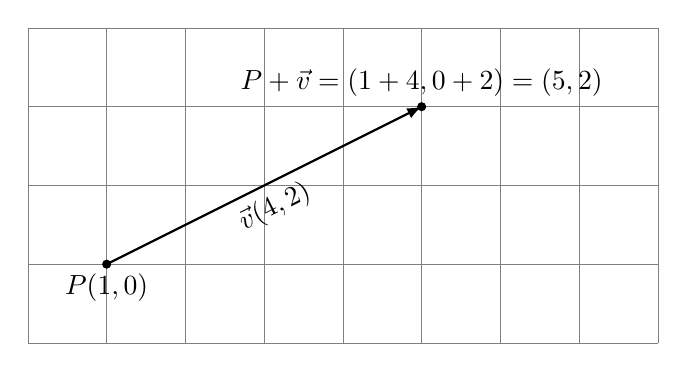
\begin{tikzpicture}
  \draw[help lines] (0,-1) grid (8,3);

  \coordinate (p1) at (1,0);
  \coordinate (p2) at (5,2);

  \draw[fill=black] (p1) circle [radius=0.05cm] node[below]{$P(1,0)$};
  \draw[thick,-latex] (p1) -- (p2) node[below,midway,sloped] {$\vec v(4,2)$};
  \draw[fill=black] (p2) circle [radius=0.05cm] node[above]{$P + \vec v = (1 + 4, 0 + 2) = (5, 2)$};
\end{tikzpicture}

\end{document}